\chapter{Heritage of ice reservoirs}

\cleanchapterquote{Before the artificial glacier, we struggled to get any barley. But now we can grow many
  crops, even potatoes, which need to be planted earlier in the spring, but sell for much more money.
}{Tashi Tundup}{(A 76 year old farmer in Ladakh)}

This chapter provides conclusions based on research findings from data collected on AIRs in Switzerland and India,
as well as discussion and recommendations for future research. This Chapter will review the purpose of the
study, research questions, literature review, and findings of the study. It will then present conclusions,
discussion of the conclusions, and recommendations for practice and for further research.

\section{Summary}

Cryosphere fed irrigation networks are completely dependant on the timely availability of meltwater from
glaciers, snow and permafrost. With the accelerated decline of glaciers, these irrigation networks can no longer
deliver adequate water to sustain agricultural output and take advantage of the complete growing season. As a
consequence, some mountain villages have either been abandoned or lie on the brink of desertification
\cite{grossmanHimalayanGlaciersMelt2015}.

In the past few decades, artificial ice reservoir (AIR) technologies have provided much needed relief to these
water-stressed communities. These strategies revolve around augmenting their glacial ice reservoirs with
man-made ones that provide supplementary irrigation during the spring. In the context of the observed present
and predicted global glacier shrinkage, the development of such water storage technologies is crucial to ensure
continued sustenance of cryosphere-fed irrigation networks.

AIR observations and investigations date back to the mid-2000s \cite{tveitenGlacierGrowingLocal2007}. The vast
majority have been published in the 2010s, mostly using qualitative methods. However, quantifications of their
storage capacity differ widely amongst these publications. \citep{baglaArtificialGlaciersHelp1998,
norphelSnowWaterHarvesting2015, nusserSociohydrologyArtificialGlaciers2019}. Because small-scale processes,
complex feedbacks and non-linearities govern their evolution, modelling the volume evolution of ice stupas is
only feasible if backed up with comprehensive input, calibration and validation datasets.

In response, we conducted measurement campaigns using drones, flowmeters and weather stations on almost a dozen
AIRs across two locations (India and Switzerland), over four winters (2019, 2020, 2021 and 2022) and using two
different construction methods (traditional and automated). Each dataset contained information on the
meteorological conditions, fountain characteristics and AIR volume evolution. 

The primary objective of this thesis was to improve our understanding about the response of AIRs to changes in
their construction location. The secondary objective was to improve the water-use efficiency and reduce its
maintenance requirements.  

\section{Conclusions}

\begin{figure}[htb]
	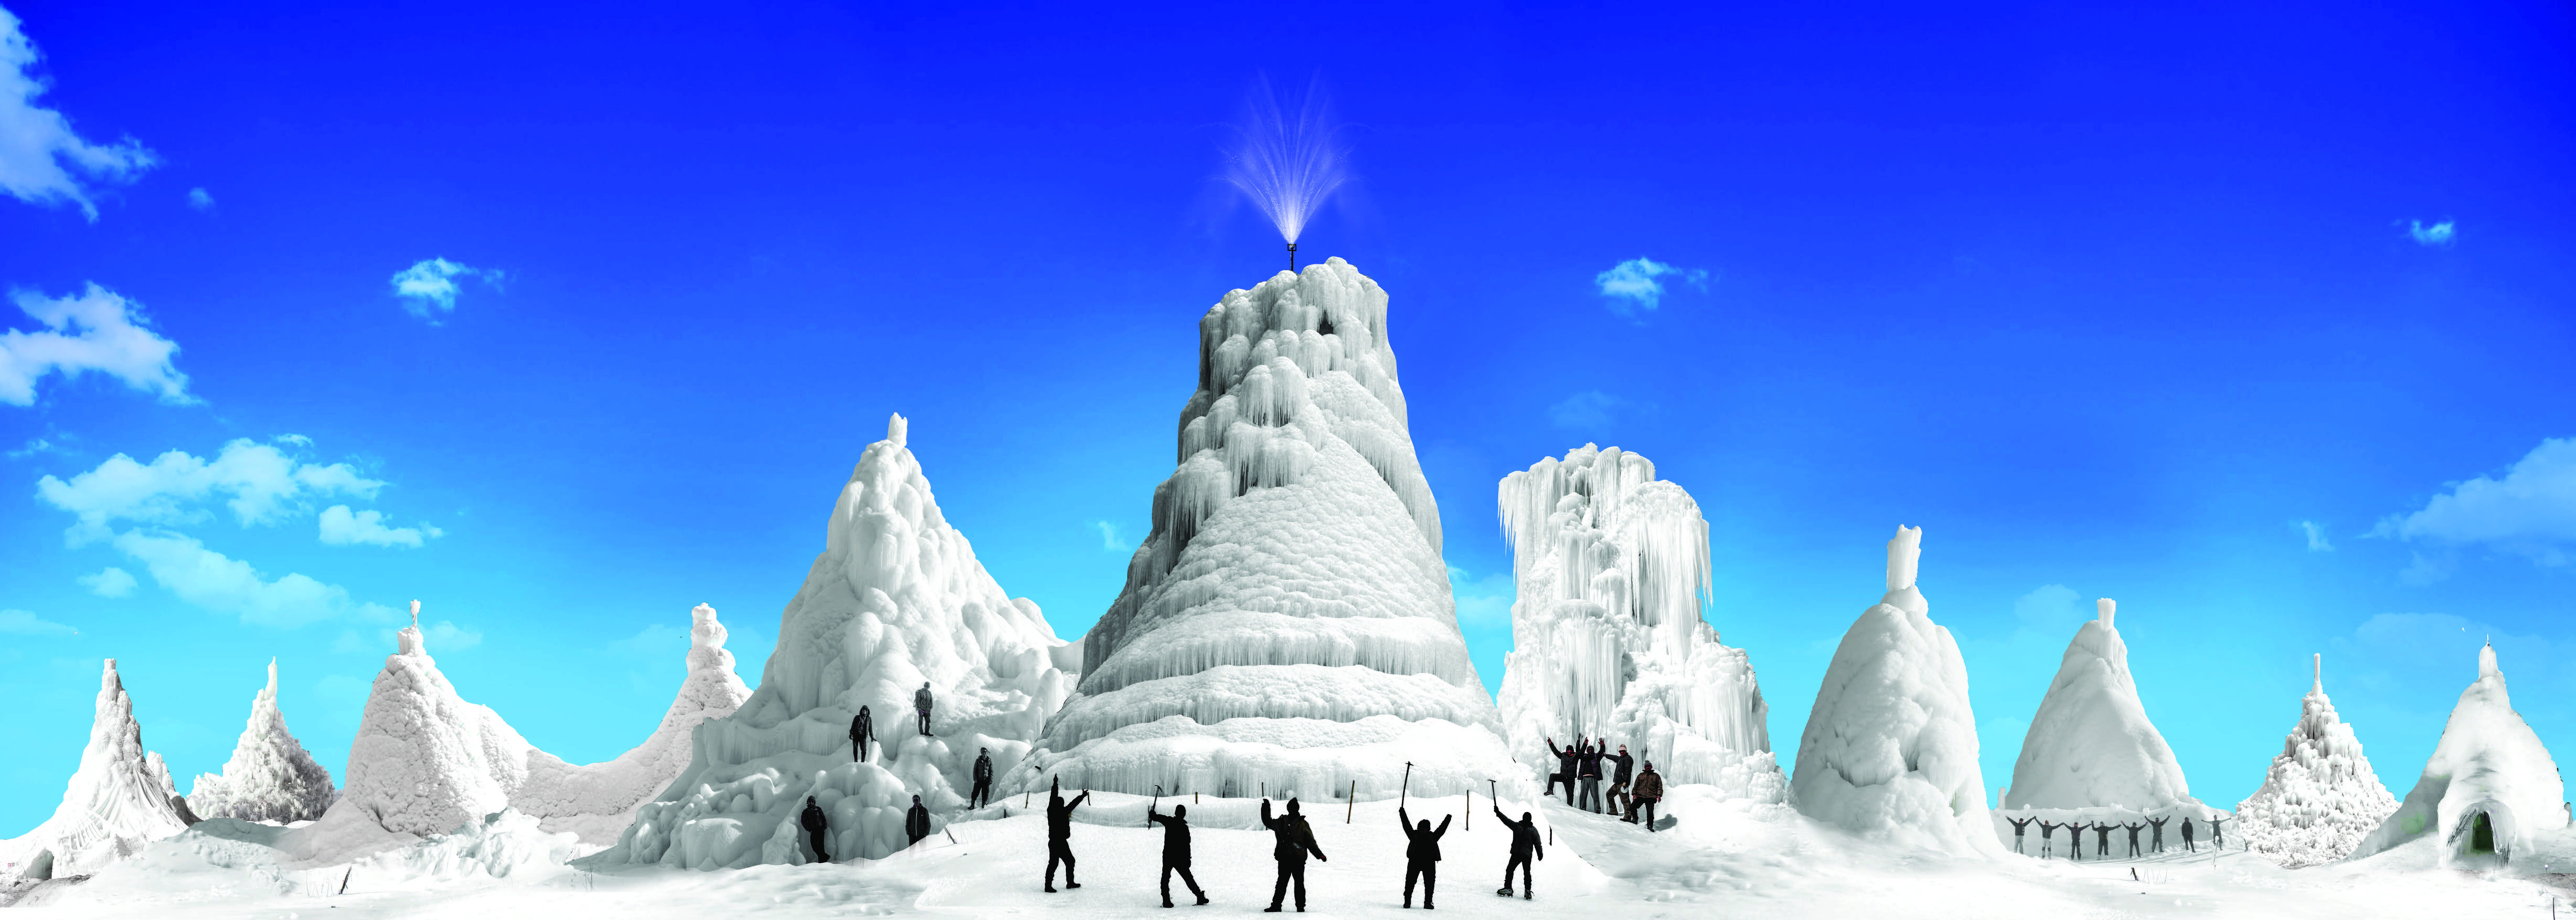
\includegraphics[width=\textwidth]{figs/AIRs_Ladakh}
	\caption{Compilation of AIRs built in different villages of Ladakh.}
	\label{fig:airs_ladakh}
\end{figure}

In paper I and II, an AIR model was designed to resolve AIR surface processes. In paper II, the modelled volume
evolution of AIRs in Indian Himalayas and the Swiss Alps were compared. In paper III, the evolution of AIRs
using different fountain scheduling strategies were compared. The results of these papers can be summarised as
follows:

\begin{enumerate} 

\item Volumes of ice stupas located in different regions may differ by an order of magnitude. The differences
  could be attributed to the accelerated sublimation process in colder and drier regions.

\item Water losses of ice stupas may be upto 80 \% due to excessive use of water by traditional construction
  strategies. However, weather-sensitive fountain systems can produce icestupas of similar volumes by using just
  one-tenth of the water supply.

\item Traditional construction strategies demand significant maintenance efforts since they are prone to
  freezing events in the fountain pipeline. However, automated construction strategies can prevent these events
  to make the construction process maintenance-free.

\end{enumerate}

\section{Discussion}

\section{Recommendations}

\section{Suggestions for future research}

\begin{itemize} 

\item Identification of favourable locations.

\item Cosistupa model development.

\end{itemize}

\section{Final thoughts}


% With a special focus on ice stupas, a mass and energy balance model was developed and used as a tool to quantify
% the influence of meteorological conditions and fountain characteristics. The meteorological and fountain
% observations were used as model input; AIR volume observations were used to calibrate the model parameters and
% validate its ice volume estimations.

% The model has been shown to perform excellently when calibrated with the AIR datasets.  It could be shown that
% the maximum volume of AIRs located in the IN and CH regions differ by an order of magnitude. These differences
% were caused by the stronger sublimation process due to the colder and drier weather conditions of the IN region. 

% AIR maintenance requirement was reduced and their fountain freezing events were prevented by developing an
% automated construction strategy. Fountain operation was made 8 times more efficient and effortless through the
% use of an automation system that scheduled discharge rates based on the recommendations of the AIR model. 

% \begin{itemize} 

% \item[\tiny{$\blacksquare$}] Colder, drier and less cloudy construction locations form long-lasting AIRs with
%   higher maximum ice volumes. 

% \item[\tiny{$\blacksquare$}] Weather-sensitive fountain systems produce larger and efficient AIRs effortlessly. 

% \end{itemize}
